% vim: set tw=78 sts=2 sw=2 ts=8 aw et ai:
\documentclass[12pt]{article}

\usepackage[paper=a4paper, top=2cm, bottom=3cm, left=2.5cm, right=2.5cm]{geometry}

\usepackage{ucs}
\usepackage[utf8x]{inputenc}
\usepackage[english]{babel}
%\usepackage{hyperref}	  % use \url{http://$URL} or \href{http://$URL}{Name}
\usepackage{underscore}	  % underscores need not be escaped
\usepackage{subfigure}
\usepackage{verbatim}
\usepackage{float}
\usepackage{booktabs}     % professional tables

% Support for including graphics
\usepackage{graphicx}
\DeclareGraphicsExtensions{.pdf,.png,.jpg}

\usepackage{color}
\usepackage{listings}
\lstset{ %
language=C++,                % choose the language of the code
basicstyle=\footnotesize,       % the size of the fonts that are used for the code
numbers=left,                   % where to put the line-numbers
numberstyle=\footnotesize,      % the size of the fonts that are used for the line-numbers
stepnumber=1,                   % the step between two line-numbers. If it is 1 each line will be numbered
numbersep=5pt,                  % how far the line-numbers are from the code
backgroundcolor=\color{white},  % choose the background color. You must add \usepackage{color}
showspaces=false,               % show spaces adding particular underscores
showstringspaces=false,         % underline spaces within strings
showtabs=false,                 % show tabs within strings adding particular underscores
frame=single,           % adds a frame around the code
tabsize=2,          % sets default tabsize to 2 spaces
captionpos=b,           % sets the caption-position to bottom
breaklines=true,        % sets automatic line breaking
breakatwhitespace=false,    % sets if automatic breaks should only happen at whitespace
escapeinside={\%*}{*)}          % if you want to add a comment within your code
}

\title{Hive - Wireless Sensor Networks simulator}

\author{Catalina Macalet, Sorin Dumitru\\
Automatic Control and Computers Faculty\\
University POLITEHNICA of Bucharest\\
Splaiul Independenței nr. 313, Bucharest, Romania \\
\emph{\{catalina.macalet,sorin.dumitru\}@cs.pub.ro}}

\date{\today}

\begin{document}

\maketitle

\begin{abstract}
% vim: set tw=78 sts=2 sw=2 ts=8 aw et ai:
This paper describes \textit{Hive}, a Wireless Sensor Nodes Network simulator.
\textit{Hive} is component based and highly scalable allowing simulations
of thousands of nodes.

It provides a standard library based on events for developing applications
for Wireless Sensor Nodes. It abstracts architecture, network protocols and
components in order to provide portability.

\end{abstract}

\section{Introduction}
\label{sec:introduction}
% vim: set tw=78 sts=2 sw=2 ts=8 aw et ai:
\textit{Hive} is a Wireless Sensor Network Simulator that is intended to be
used for simulating routing protocols for Wireless Sensors Networks in order
to determine the best suited protocol for a given topology.
There exist a number of simulators used for simulating Wireless Sensor
Networks such as NS-2, J-sim\cite{jsim-article} and TOSSIM\cite{tossim}. We will not go into details regarding
these simulator since this was covered in our previous work. What is to be
noted though is that, after the survey we did on these simulators, we were able
to define some key features that we wanted the \textit{Hive} simulator to
have, such as, but not limited to: to be component based in order to make it easy to extend and to make future development easier to
be done, to be able to simulate a wide variety of nodes in order to not be
limited to only some sensors types, to make it easy to write code that is to
be run on nodes in order to make the implementation of the routing protocols
easier to be done and, after looking at the trends in the Wireless Sensor
Networks research, we decided that the simulator should, in the begining
support at least the 6LoWPAN and ZigBee protocol stacks.
Also, unlike some of the simulators enumerated above, \textit{Hive} targets topologies of Wireless Sensor
Networks and so, during the desing and implementation phases decisions were
made so that \textit{Hive} could simulate as accurate as possible a real
sensor.

The structure of the paper is at follows: in section 2 we present the
\textit{Architecture} of the \textit{Hive} simulator, discussing the reasons for which such
an architecture was chosen and present the communication mechanisms between
the components. Then, the \textit{Implementation} section follows where we briefly present
the libraries and tools used for implementation and the reasons for which we
chose to use these and, also, go into some details concerning the implementation.
In section \textit{Testing} we present the tests we want to do in
order to test the way \textit{Hive} behaves and to be able to provide some
numbers for the scalability matter.
In the end some conclusions are drawn, and the next steps are highlighted in
the \textit{Conclusions and Further Work} section. 


\section{Architecture}
\label{sec:architecture}
% vim: set tw=78 sts=2 sw=2 ts=8 aw et ai:

A wireles sensor node node running in a Hive simulation is 
represented by a dynamic library, which we will call plugin. This library contains the code 
which would normally run on the node, with a few simple extra methods
so it it can be used in the simulator. This library will be loaded once
for each node type.

The plugin will set timers to schedule work on the node. Lets say that we have
a node with two sensors, a temperature sensor and a noise sensor. Upon
initialisation, the sensor will set a timer to run once every 5 minutes to
read temperature and another one for the noise sensor to run once every
minute. The plugin will collect the data from these sensors in internal memory
and set a timer to send the data to a master node once every 30 minutes.

\subsection{Networking}

The Hive simulator has support for the 6LowPAN and ZigBee protocols.

\subsubsection{6LowPAN\cite{6lowpan}}
A LoWPAN is a simple low cost communication network that allows
wireless connectivity in applications with limited power and relaxed
throughput requirements.  A LoWPAN typically includes devices that
work together to connect the physical environment to real-world
applications, e.g., wireless sensors.  LoWPANs conform to the IEEE
802.15.4-2003 standard.


\subsubsection{Zigbee}
ZigBee is a technology used in automation and remote control applications that
provides low data rate, low power, low consumption wireless networking. It is mainly
used in equipments that require long battery life but not high transfer rate as those
enabled by Bluetooth.
Zigbee uses the functionality and standardisation of the physical layer and
medium access control layer de?ned in IEEE 802.15.4 for LoWPANs to which it then adds
a couple of layers: the network layer, and the application layer and two main
components: the ZigBee device objects (ZDOs) and manufacturer-defined application objects.
The last two components allow customization of applications which could de?ne
their own behaviours and, also, total integration.

\begin{figure}[htb]
  \begin{center}
    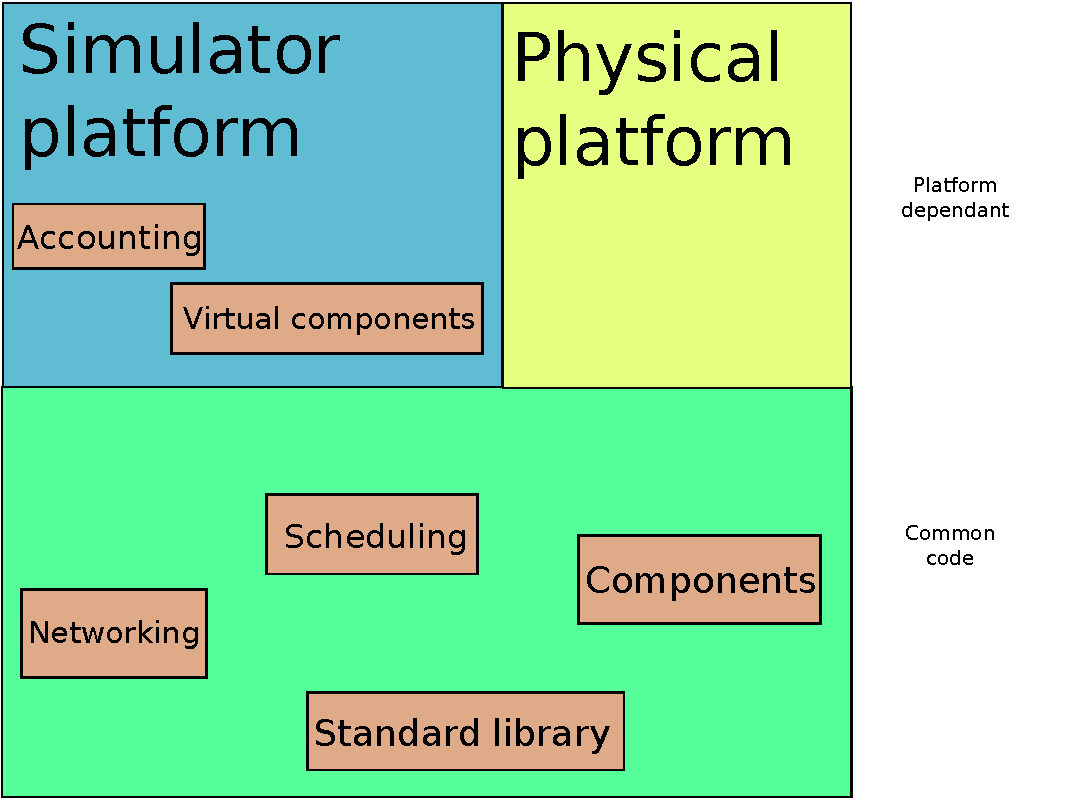
\includegraphics[scale=0.75]{img/bigarch.pdf}
    \caption{Hive simulator Architecture}
  \end{center}
\end{figure}


\subsection{Controlling the simulator}

The simulator is controlled through simple commands on a TCP socket. For
example to load a test plugin, start it, stop it and then unload it we would
do:
\begin{lstlisting}
$ nc 127.0.0.1 54321
load test
1
start 1
stop 1
unload 1
\end{lstlisting}

If the library test.so is not found in LD_LIBRARY_PATH an error will be
thrown.


\section{Implementation}
\label{sec:implementation}
% vim: set tw=78 sts=2 sw=2 ts=8 aw et ai:

The \textit{Hive} simulator is implemented in a mix of C and C++. C is used in the core
library that will also be used on physical nodes. C++ is used in the
simulator so we can use the Standard Template Library. While C++ could also be
used on a node, it consumes more memory than C and the nodes usually do not
have too much memory.

\subsection{Standard library}

In order for the wireless sensor nodes to be useful they will have to be
programmed to do a certain task. For this, \textit{Hive} provides an API. It allows
common tasks like scheduling a timer or creating sockets. 

This API provided by \textit{Hive} is platform agnostic. The code is loadable in the
simulator as a plugin using \textit{libdl}. When used on a physical node, the plugin must
provide only a load routine. When ran on the simulator platform, the plugin
should also provide a start, stop and unload routine.

\subsection{Networking}

\textit{Hive} provides an API similar to the BSD sockets one. The functions name are
all appended with sys so they do not collide with the ones from glibc. The API
contains just a small subset of BSD sockets one, but it will be extended if needed.
\begin{lstlisting}
sys_socket(int type, int protocol);
sys_sendto(int sock, char *buff, int size, sockaddr *to)
sys_recvfrom(int sock, char *buff, int size, sockaddr *from);
\end{lstlisting}
The plugin needs to specify the protocol used only when the socket is created,
but for all subsequent calls this will be handled by internal systems. 

\begin{figure}[htb]
  \begin{center}
    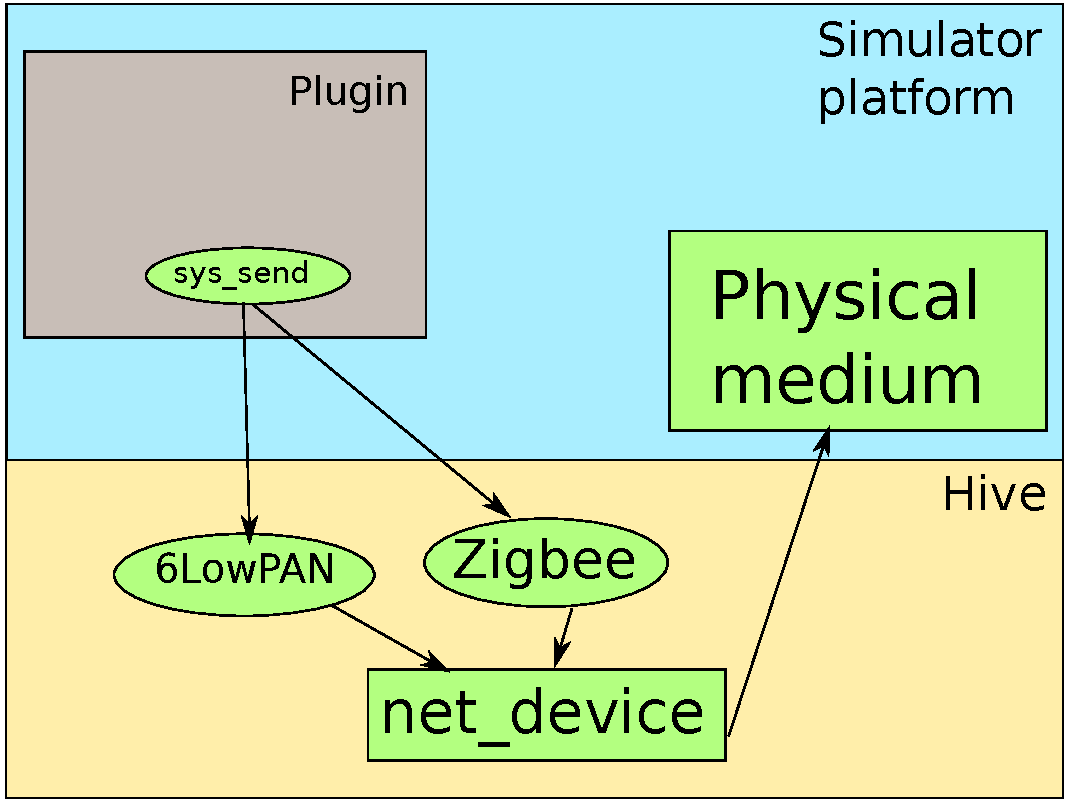
\includegraphics[scale=0.75]{img/networking.pdf}
    \caption{Network packet flow}
  \end{center}
\end{figure}

The flow of a network packet will start in the plugin. It will create a socket
using sys\_socket and will be able to send data using sys\_sendto. In the
networking system a packet will be created in which the data from the buff
argument will be copied. This packet will be passed to the protocol for this
socket which will add the protocol specific headers to it based on internal
structures. When the protocol is done with the packet, the packet is passed to a
driver for a network device.

On a physical node, the network device driver will send the packet to the
destination node using WiFi, radio, etc. On the simulator platform, the
packet is passed back to the simulator which maintains a packet queue for each
node and will route the packet to the appropriate node.

On the receive side, the simulator periodically checks the receive packet
queues for nodes and sends a notification to the node to start processing a
packet if one was received.
The packet will go through the network device driver, which will pass it to
the protocol which will then pass it to the plugin after removing all headers.

\subsection{Scheduler}

Most of work on a wireless sensor node is triggered by an event. For example
we read the temperature sensor every 5 minutes, which is a timer event, or an
actual event happens on the node, for example a packet arrives.

The job of the scheduler is to provide a way to register for and notify of
events. The scheduler is split in two parts: a platform agnostic one and a platform
specific one. The platform agnostic part contains the API needed by users in
order to to use the scheduler. It allows specifing callbacks for events or timers:

\begin{lstlisting}
typedef void (*callback_t)(void *arg);
void schedule_timer(struct scheduler *scheduler,
                    /* Timeout in miliseconds *?
                    int timeout, 
                    /* Callback function */
                    callback_t *cb, 
                    /* Argument to be passed to the callback */
                    void *arg);
\end{lstlisting}
The platform specific part contains the platform dependent implementation of
the scheduler. Each platform has a different implementation for timers so each
platform will have to implement its own version of this part. For example Linux has
timerfds, but an Atmega microcontroller has hardware timers. The scheduler
implementation for that platform will use the functions and functionality that the platform provides.

The implementation of the scheduler on the simulation platform will be done
using libevent\cite{libevent} library. The libevent API provides a mechanism to execute a callback
function when a specific event occurs on a file descriptor or after a timeout
has been reached. Furthermore, libevent also support callbacks due to signals
or regular timeouts. Libevent uses the event loop mechanisms provided by the
system on which it runs. This can be /dev/poll, kqueue, select, event ports,
poll, epoll.

\subsection{Accounting}

The Accounting component is needed to get some information about the
status of the sensor: the battery status, the predicted lifetime of the
sensor, etc. 

Everything that runs on a node consumes some power and the simulator will have
to reflect that in the battery level of the node. For example reading a sensor
will consume a small part of the battery while sending messages to a node will
consume much more power, depending on the distance of the target node from the
source node.

Every event on a simulated node will pass one or more times through the
scheduler. This will happen either as a normal timer event or from the simulator
part of the driver for the component. If a timer expires, we call the callback
function which means the node is running some code and we will be able to
estimate how much battery it consumes based on the time the callback takes.
For a network packet we will be able to do the accouting when the packet
reaches the physical layer of the simulator where it will be able to compute
the power consumption to communicate with the target node.


%\section{Experimental Setup}
%\label{sec:setup}
%% vim: set tw=78 sts=2 sw=2 ts=8 aw et ai:

In order to define recursion, one must first define recursion.


%\section{Scenarios and Results}
%\label{sec:results}
%% vim: set tw=78 sts=2 sw=2 ts=8 aw et ai:

The end justifies the means.


\section{Testing}
\label{sec:testing}
% vim: set tw=78 sts=2 sw=2 ts=8 aw et ai:

The \textit{Hive} simulator is not yet in a state where we can do testing on
it and get reliable results but  we intend to test each of its features; here
we outline our plans for testing the simulator.

\begin{itemize}
	\item \textit{API testing} will be done using a simple protocol
	which uses as source and destination nodes the nodes ids. This will be used
	for testing changes to the API as the network system will not
	have too much work to do for this simple protocol.
	\item The second test phase will be to \textit{test each of the
        supported protocols}. Packets
	will be dumped to a file and analyzed to see if they conform
	to the specifications of the protocols.
	\item \textit{Scalability} - We want to know how many nodes
	the simulator will be able to simulate. We also
	intend to do profiling on these tests to see where the simulator
	spends most of the time and, after investigating this, to decide if we can further improve it.
	\item \textit{Node complexity} We also want to see how
	many nodes doing complex things \textit{Hive} can simulate. This
	will be done with infinite battery and doing high network
	traffic.
\end{itemize}


\section{Conclusion and Further Work}
\label{sec:conclusion}
% vim: set tw=78 sts=2 sw=2 ts=8 aw et ai:
\textit{Hive} is a Wireless Sensor Network simulator incorporating some of the
key design features of some of the surveyed simulators: it has a component
based architecture, uses a modular implementation, it is easy to use by being
able to control its actions over a TCP-socket by using a simple list of
commands as shown in section \textit{2.1 Controlling the simulator}.
It is written in C and C++ and uses a portable library (libevent) to handle
events in order to make the whole simulator easy to port on other platforms
than Unix.

The desing of the \textit{Hive} simulator provides an easy-to-use interface
for adding support for other protocol stacks and also for adding new types of
nodes by defining values for sensor properties such as power, CPU, resources
consumed when sending/receiving a message, etc making it a useful tool for
research purposes.
%porting to other platforms
The effort needed to port \textit{Hive} simulator to another platform should
not be too big since the changes are limited to the physical platform
code-area.

%testing
The first thing that needs to be completed at this stage before adding more
functionality or improving usabilitity is finishing the testing phase. It is
important to establish the way \textit{Hive} simulator behaves both from the
functionality point of view but also, from a scalability point of view.

%tools for viewing the traffic
Then it would be very useful to have a traffic tool for capturing and
analyzing the traffic from the Wireless Sensor Network. This needs also to be
added and it could easily be implemented by adding a hook at
the physical layer level of the simulator.

%implementing routing protocols
The final step that needs to be acomplished in order for \textit{Hive} to be fully
functional is adding a routing protocol support for the Wireless Sensor
Network and analyzing the results.

%GUI
A features that would increase \textit{Hive}'s usability is a GUI: at first
providing basic functionality such as permiting the selection of nodes
or componet types and adding them in a 2D space and, later, at a more developed phase, it could
permit to create a more realistic scenario by incorporating obstacles, natural
phenomena, etc.


\section*{Acknowledgment}
\label{sec:acknowledgment}

The authors would like to thank XYZ for their support and dedication.

\bibliographystyle{abbrv}
\bibliography{my-report}

\end{document}
